\documentclass[dvipdfmx]{standalone}
\usepackage{tecfig}
\usepackage{myFlowChart}
\begin{document}
	\begin{tikzpicture}
		\def\largearrow#1#2{

			\coordinate (arrow#1-left)  at ($(#2) - (0.75, 0)$);
			\coordinate (arrow#1-right) at ($(#2) + (0.75, 0)$);

			\draw (arrow#1-left)  -- ++( 0.25,  0.25) coordinate (al-above);
			\draw (arrow#1-left)  -- ++( 0.25, -0.25) coordinate (al-below);
			\draw (arrow#1-right) -- ++(-0.25,  0.25) coordinate (ar-above);
			\draw (arrow#1-right) -- ++(-0.25, -0.25) coordinate (ar-below);

			\draw ($(arrow#1-left)!0.5!(al-above)$) -- ($(arrow#1-right)!0.5!(ar-above)$);
			\draw ($(arrow#1-left)!0.5!(al-below)$) -- ($(arrow#1-right)!0.5!(ar-below)$);
		}
		\node[align=center, draw, anchor=south] (CPU) at (0, 6.5*1.4) {CPU\\(計算,制御)};
		\draw ($(0, 0)-(0.5, 0)$) rectangle ($(CPU.south)+(0.5, 0)$);
		\node[align=center, draw, anchor=west] (memory) at (2, 6*1.4) {主記憶装置/メモリ\\(256バイト)};
		\node[align=center, draw, anchor=west] (interface1) at (2, 5*1.4) {インタフェース回路};
		\node[align=center, draw, anchor=west] (interface2) at (2, 4*1.4) {インタフェース回路};
		\node[align=center, draw, anchor=west] (interface3) at (2, 3*1.4) {インタフェース回路};
		\node[align=center, draw, anchor=west] (interface4) at (2, 2*1.4) {インタフェース回路};
		\node[align=center, draw, anchor=west] (interface5) at (2, 1*1.4) {インタフェース回路};
		
		\largearrow{7}{[xshift=-0.75cm]memory.west};
		\largearrow{1-1}{[xshift=-0.75cm]interface1.west};
		\largearrow{2-1}{[xshift=-0.75cm]interface2.west};
		\largearrow{3-1}{[xshift=-0.75cm]interface3.west};
		\largearrow{4-1}{[xshift=-0.75cm]interface4.west};
		\largearrow{5-1}{[xshift=-0.75cm]interface5.west};
		
		\largearrow{1-2}{[xshift=0.75cm]interface1.east};
		\largearrow{2-2}{[xshift=0.75cm]interface2.east};
		\largearrow{3-2}{[xshift=0.75cm]interface3.east};
		\largearrow{4-2}{[xshift=0.75cm]interface4.east};
		\largearrow{5-2}{[xshift=0.75cm]interface5.east};

		\node[anchor=west, inner sep=0pt] (timer) at (arrow1-2-right) {
			\begin{tikzpicture}
				\draw (0, 0) circle[radius=0.6cm];
				\draw[-latex] (0, 0) -- (0, 0.6);
			\end{tikzpicture}
		};
		
		\node[anchor=west, inner sep=0pt] (serial) at (arrow2-2-right) {
			\begin{tikzpicture}
				\node[draw, align=center, inner sep=2pt] at (0, 0) {シリアル通信};
			\end{tikzpicture}
		};
		
		\node[anchor=west, inner sep=0pt] (speaker) at (arrow3-2-right) {
			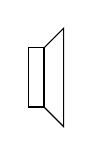
\begin{tikzpicture}
				\draw (0, 0) rectangle (0.2, 0.75);
				\draw (0.2, 0) -- ++(0.25, -0.25) -- ++(0, 1.25) -- ++(-0.25, -0.25);
			\end{tikzpicture}
		};
		
		\node[anchor=west, inner sep=0pt] (data-switch) at (arrow4-2-right) {
			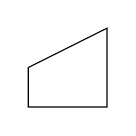
\begin{tikzpicture}
				\draw (0, 0) -- (0, 0.5) -- (1, 1) -- (1, 0) -- cycle;
			\end{tikzpicture}
		};

		\node[anchor=west, inner sep=0pt] (io-port) at (arrow5-2-right) {
			\begin{tikzpicture}
				\node[draw, align=center, inner sep=2pt] at (0, 0) {入出力ポート};
			\end{tikzpicture}
		};

		\node[anchor=west, align=center] at (timer.east) {タイマ};
		\node[anchor=west, align=center] at (speaker.east) {スピーカ};
		\node[anchor=west, align=center] at (data-switch.east) {データ\\スイッチ};
		
		\coordinate (io-inter) at ($(interface5.south) + (0, -1)$);
		\coordinate (io-equip) at ($(interface5.south) + (4.5, -1)$);

		\draw[dashed] ($(io-inter) - (2, 0)$) rectangle ($(io-inter) + (2, 5.4 * 1.4)$);
		\draw[dashed] ($(io-equip) - (2, 0)$) rectangle ($(io-equip) + (2, 5.4 * 1.4)$);
		\node[anchor=north] at (io-inter.south) {入出力インターフェース};
		\node[anchor=north] at (io-equip.south) {入出力装置};
		
		\node[rotate=-90] at (0, 6) {バス};
		
		

	\end{tikzpicture}
\end{document}
